\section{Cryogenic System and Gas Purification}
\label{secGasSystem}

%The xenon gas for the XENON100 detector is stored in four high pressure aluminum cylinders, shown in Fig.~\ref{figGasRack}. They can be immersed in the dewars with $\sim$70~l capacity, and cooled down with liquid nitrogen, in order to recover xenon from the detector. 

%\begin{figure}[!h]
%\centering
%\subfigure[]{
%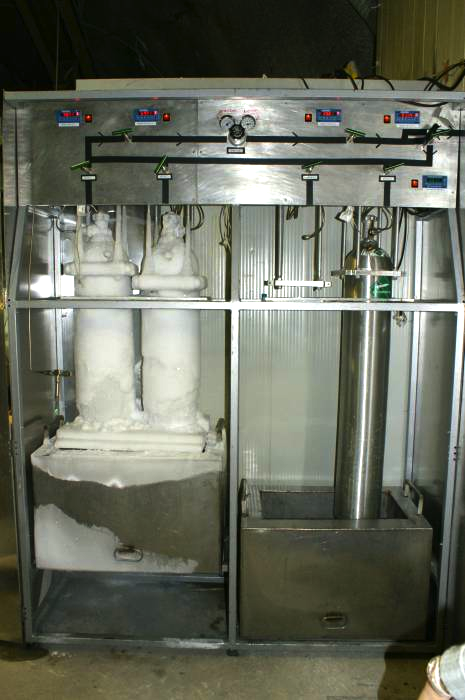
\includegraphics[height=0.5\linewidth]{plots/Detector/GasRack.png}
%\label{figGasRack_1}}
%\subfigure[]{
%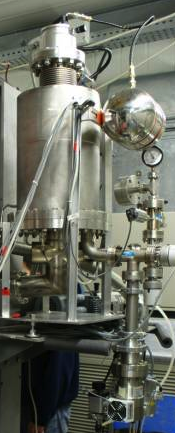
\includegraphics[height=0.5\linewidth]{plots/Detector/CoolingTower_door.png}
%\label{figGasRack_2}}
%\subfigure[]{
%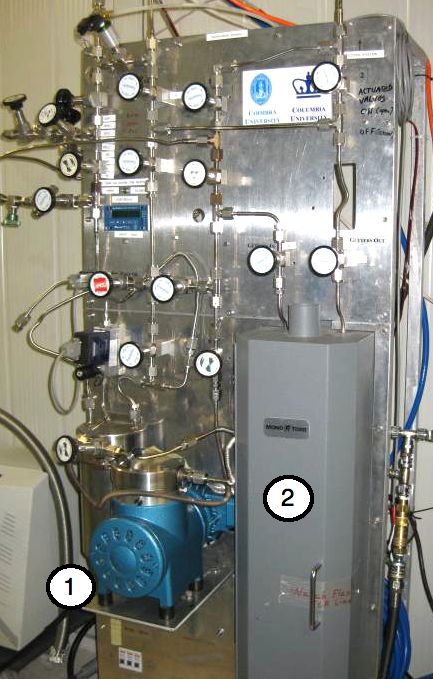
\includegraphics[height=0.5\linewidth]{plots/Detector/PurificationPanel_withLabels.png}
%\label{figGasRack_3}}
%\caption[The XENON100 gas system]{The XENON100 gas system. (a) - gas bottle rack during recuperation. (b) - cooling tower with a pulse-tube refrigerator (PTR) mounted on the shield door. (c) - gas recirculation and purification rack: 1 - recirculation pump, 2 - high temperature getter.}
%\label{figGasRack}
%\end{figure}


%\begin{floatingfigure}[lh]{0.3\textwidth}
%\begin{figure}[!h]
%\centering
%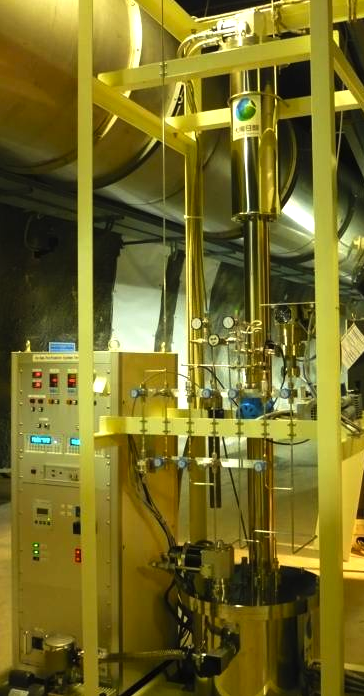
\includegraphics[height=0.6\linewidth]{plots/Detector/DistillationColumn.png}
%\caption{Cryogenic distillation column for krypton removal.}
%\label{figDistillationColumn}
%\end{figure}
%\end{floatingfigure}

%\begin{floatingfigure}[r]{0.3\textwidth}
%\begin{figure}[!h]
%\centering
%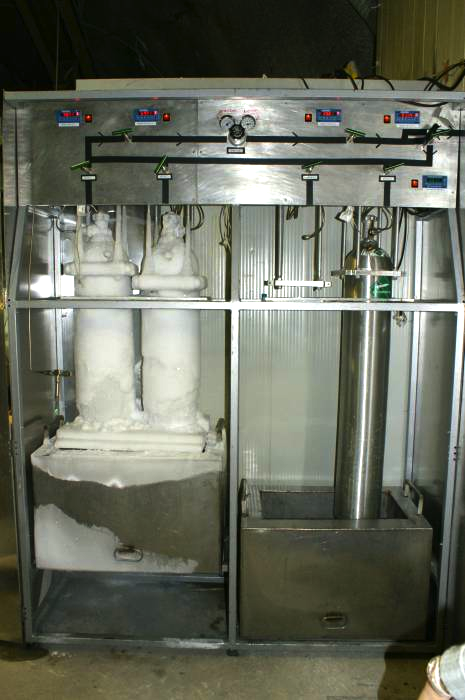
\includegraphics[width=0.3\linewidth]{plots/Detector/GasRack.png}
 %\caption{The XENON100 gas bottle rack during recuperation.}
%\label{figGasRack}
%\end{figure}
%\end{floatingfigure}

The schematic diagram of the cryogenic system of the XENON100 experiment is shown in Fig.~\ref{figCoolingTower_1}. It is based on Iwatani PC150~\cite{PTR} pulse tube refrigerator, powered by a 6.5~kW helium compressor. The measured cooling power is 200~W at 170~K, which allows the xenon gas to be liquified during the detector filling at a rate of $\sim$3~kg/hour.  The PTR is mounted together with its motor valve and buffer tank on a small double-walled vessel outside of the detector shield (Fig.~\ref{figCoolingTower_2}). The bottom of this vessel is connected to the detector cryostat with a vacuum insulated pipe, at a height above the liquid level. 
The PTR cold head is mounted on a cylindrical copper block, and then sealed to the inner vessel of the PTR cryostat with an aluminum wire, so that the PTR can be serviced or even replaced without exposing the detector volume to air. The temperature and pressure of the detector is regulated with an electric heater, which is installed in a copper cup connected to the cold head. The temperature is measured with Pt100 resistance thermometers connected to a PID controller.

When the gas from the detector reaches the cold head, it is liquefied, and the drops of liquid xenon are collected by a funnel and transferred via a 1/4-inch diameter pipe into the detector cryostat. The transfer is driven by gravity, therefore the connecting pipe is inclined by 5$^{\circ}$ to the horizontal.

\begin{figure}[!b]
\centering
\subfigure[]{
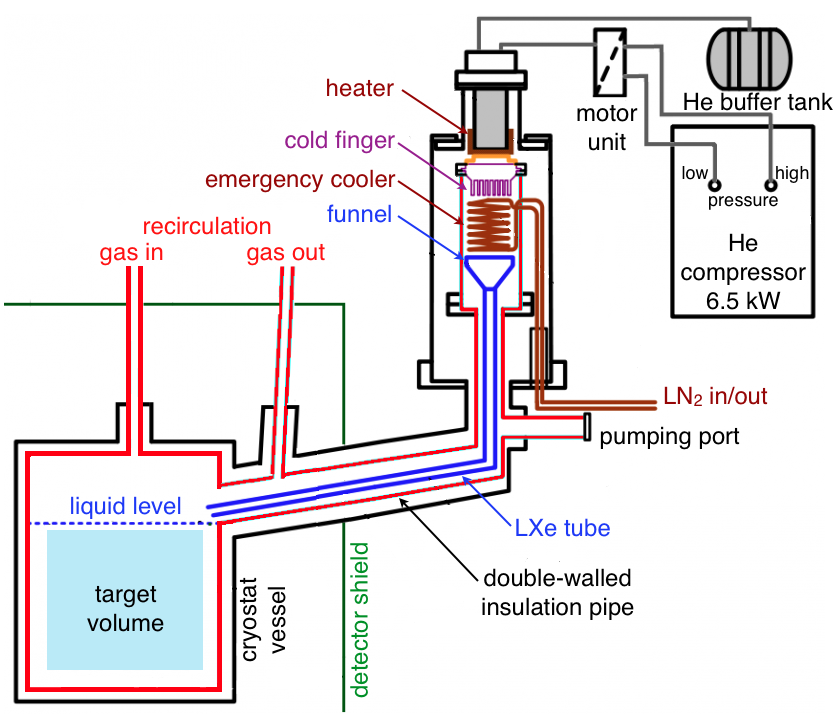
\includegraphics[height=0.6\linewidth]{plots/Detector/schemeMod_CoolingSystem.png}
\label{figCoolingTower_1}}
\subfigure[]{
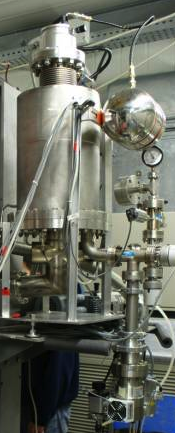
\includegraphics[height=0.6\linewidth]{plots/Detector/CoolingTower_door.png}
\label{figCoolingTower_2}}
\caption[The schematics of the XENON100 cryogenic system, and the cooling tower with pulse tube refrigerator]{The schematics of the XENON100 cryogenic system (a), and the cooling tower with pulse tube refrigerator (b). Scheme from Ref.~\cite{xe100-instrument}.}
\label{figCoolingTower}
\end{figure}

A copper coil, winded around the PTR cold head and connected to an external liquid nitrogen dewar, provides cooling in case of power outage, PTR failure, or when additional cooling power is needed in case of a loss of insulation vacuum. The external dewar is always kept full (above 80\%), and equipped with an actuated valve which is controlled via the detector pressure. This emergency system provides 48~hours of stable operation in case of a failure of the main cooling system.

Electro-negative impurities (such as oxygen) and water present in xenon gas affect the light and charge yields, respectively. In order to achieve the required electron lifetime and long VUV absorption length, their concentration has to be well below 1~parts-per-billion (ppb). The xenon purification is performed with a high temperature metal getter (MonoTorr~PS4-MT15-R-1~\cite{MonoTorr}). The continuous gas flow through the getter of 5~slpm is achieved by a diaphragm pump (KNF~N.143~\cite{KNFpump}). The gas recirculation system and its schematics are shown in Fig.~\ref{figPurificationPanel}. The xenon gas for the XENON100 detector is stored in four high pressure aluminum cylinders. In order to recover xenon from the detector, they are immersed in dewars with $\sim$70L capacity, and cooled with liquid nitrogen. 

\begin{figure}[!h]
\centering
\subfigure[]{
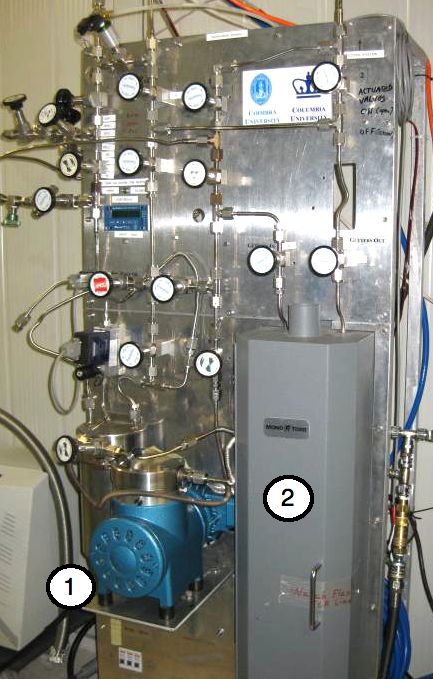
\includegraphics[height=0.55\linewidth]{plots/Detector/PurificationPanel_withLabels.png}
\label{figPurificationPanel_1}}
\subfigure[]{
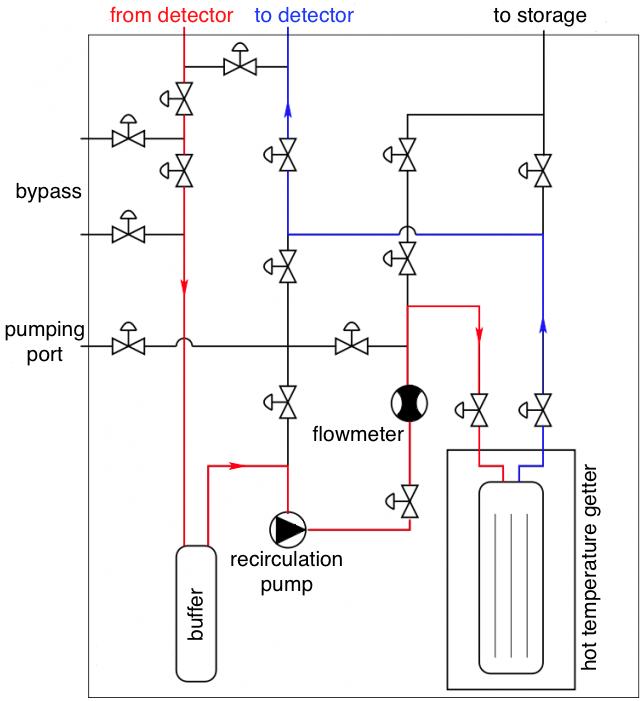
\includegraphics[height=0.55\linewidth]{plots/Detector/schemeMod_PurificationPanel.png}
\label{figPurificationPanel_2}}
\caption[The XENON100 gas purification panel]{The XENON100 gas purification panel: 1 - recirculation pump; 2 - hot getter. Scheme from Ref.~\cite{xe100-instrument}.}
\label{figPurificationPanel}
\end{figure}

Commercially available xenon gas has a concentration of krypton at the ppm level.
Natural krypton contains about 10$^{-11}$ of radioactive $^{85}$Kr~\cite{Kr85abundance_1, Kr85abundance_2}. 
The background from the beta decay of $^{85}$Kr, with half-life of 10.76~years and endpoint energy of 687~keV, is a potential limitation in the sensitivity of dark matter searches using xenon targets. 

\begin{figure}[!t]
\centering
\subfigure[]{
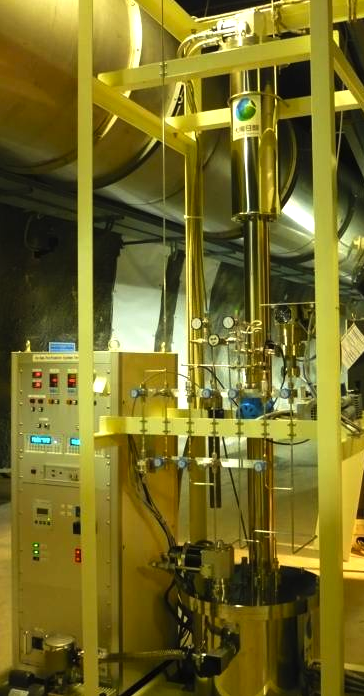
\includegraphics[height=0.6\linewidth]{plots/Detector/DistillationColumn.png}
\label{figDistillationColumn_1}}
\subfigure[]{
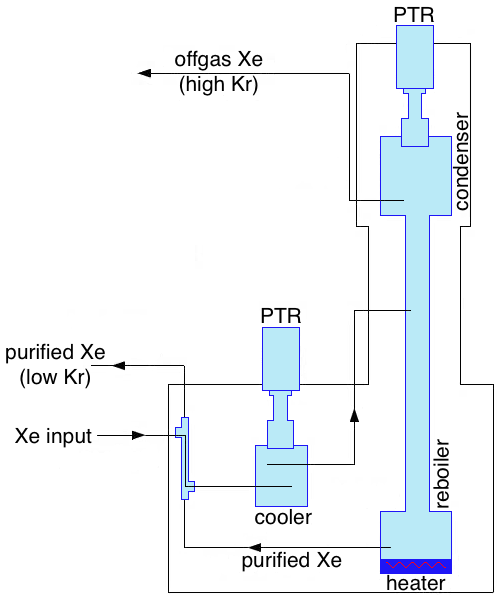
\includegraphics[height=0.6\linewidth]{plots/Detector/schemeMod_DistillationColumn.png}
\label{figDistillationColumn_2}}
\caption[Cryogenic distillation column for krypton removal]{Cryogenic distillation column for krypton removal. Scheme published in Ref.~\cite{xe100-instrument}.}
\label{figDistillationColumn}
\end{figure}

Krypton concentration in xenon can be reduced by distillation and adsorption-based chromatography methods. 
The gas used in the XENON100 experiment has been processed at a commercial distillation plant to reduce the concentration of krypton to $<$10~ppb, however, still above the XENON100 requirements of $\sim$100~parts-per-trillion (ppt) in order to reach the designed sensitivity.
The high-temperature getter used in the experiment to purify xenon from water and electronegative contaminants does not remove the noble gas krypton. Additional gas purification is achieved with a cryogenic distillation column based on the difference of the boiling points for krypton and xenon (120~K and 165~K at 1~atm, respectively). The krypton removal column has been developed by Taiyo Nippon Sanso~\cite{NipponSanso}, and is shown in Fig.~\ref{figDistillationColumn_1}. It is based on McCabe-Thiele method~\cite{McCabe} and is designed to deliver a factor of 1000 reduction of krypton concentration in a single pass. The schematic circuit is illustrated in Fig.~\ref{figDistillationColumn_2}. The main element in the distillation system is a tower in which liquid-gas equilibrium is maintained. A liquid is boiled using a heater in the `reboiler' vessel at the bottom of the tower. A condenser, placed on its top, maintains a constant temperature profile in the tower. The xenon gas is cooled down to a near boiling point and then supplied to a feed point. The processed xenon obtained from the reboiler contains a lower concentration of krypton than the original gas, and xenon with a higher krypton concentration is obtained at the top of the tower. 

The purification is performed in XENON100 with rate of $\sim$1.7~slpm, and the processing of the total amount of xenon required to fill the detector (161~kg) takes about two weeks, compared to 2-3~days needed for normal filling and recovering. The reduction of the krypton concentration down to a few ppt has been reported in Ref.~\cite{DistillationColumn}, where a small sample of processed xenon gas has been analyzed by mass spectrometry. This level of purity has not yet been achieved by XENON100 (see Section~\ref{secDelayedCoincidenceKr85}), however, this is the first large-scale experiment sensitive to such ultra-low krypton concentration.

